\begin{figure}[H]
\centering
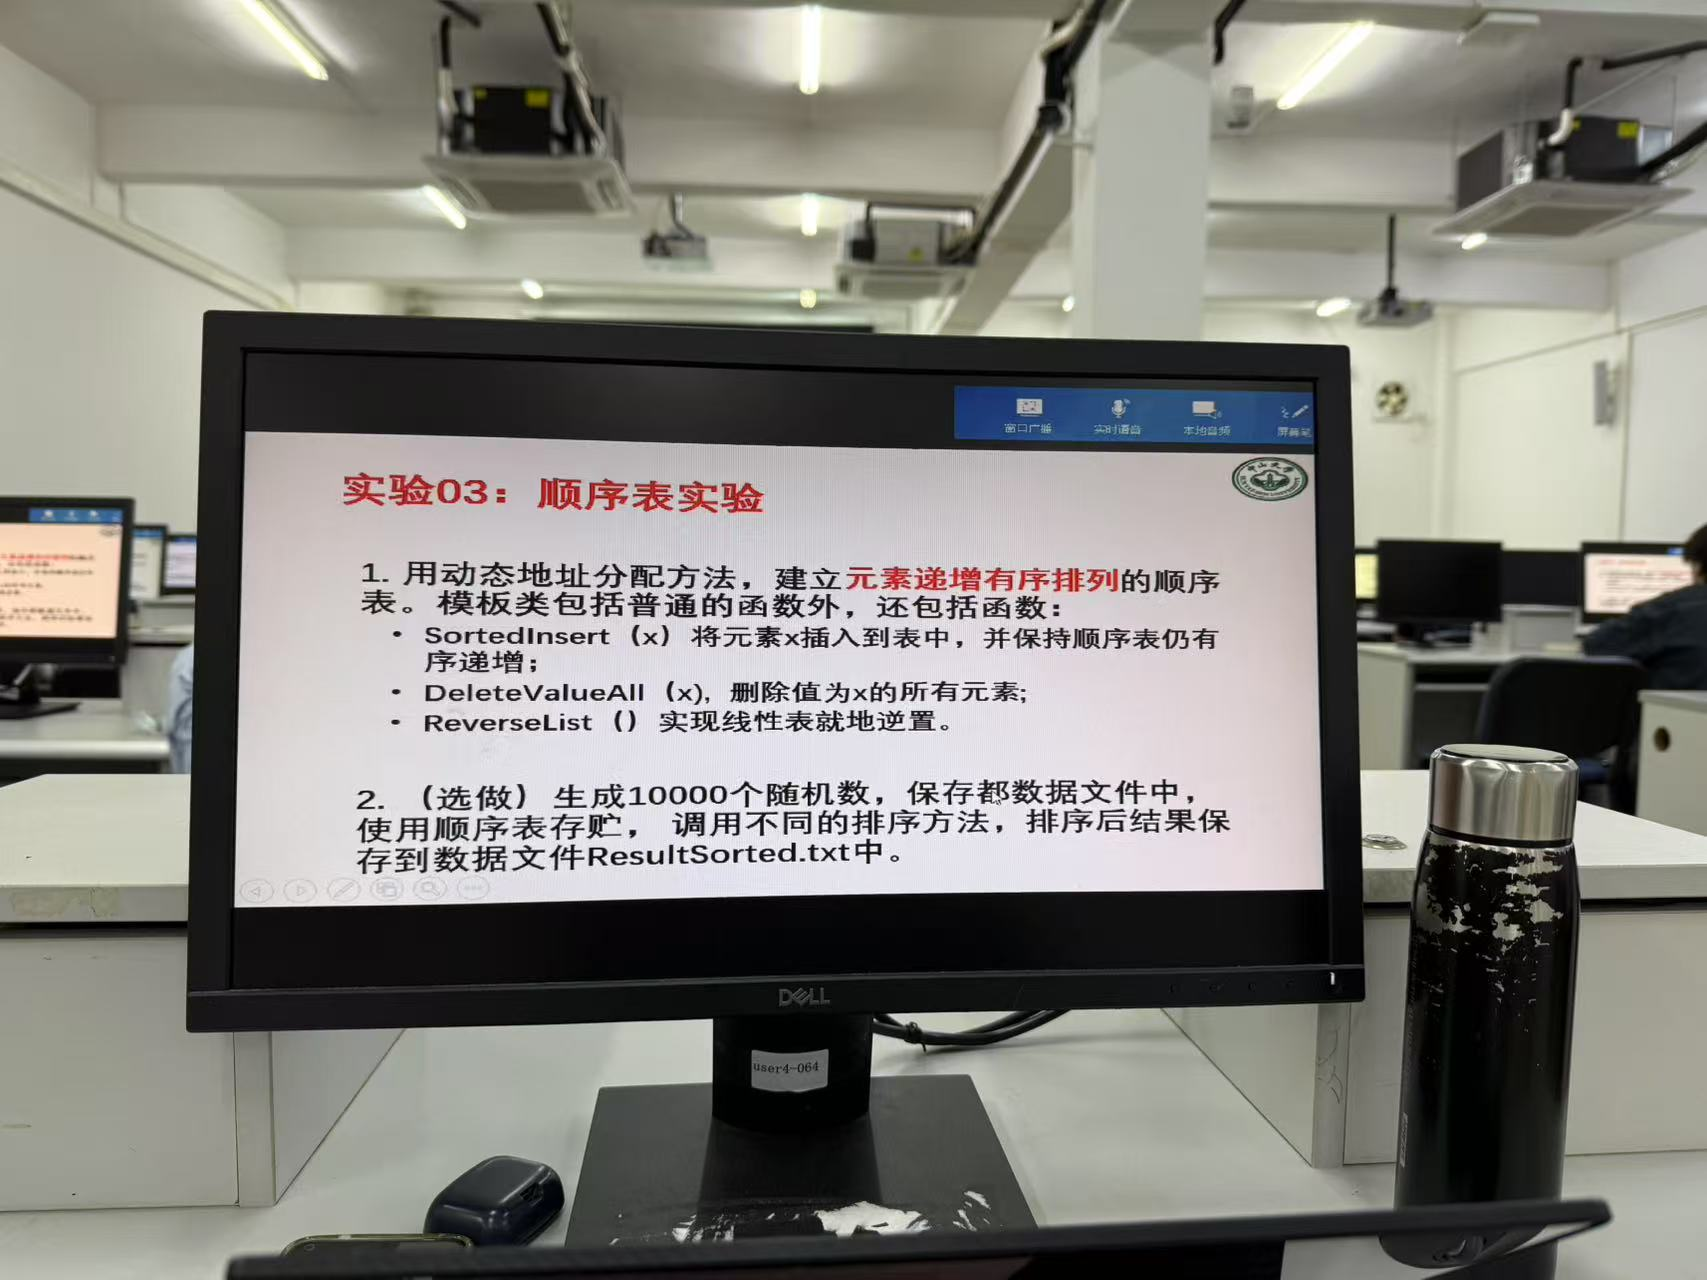
\includegraphics[width=\textwidth]{ead895c7940279838e8c65b36a36e16.jpg}
% \caption{}
\label{}
\end{figure}

\section{建立元素递增有序排列的顺序表包含函数}

\begin{lstlisting}[language=C++]
/*******************************************

   对应教材2.6.2节,顺序表的动态分配方式

********************************************/

#include <iostream>

using namespace std;

  

const int InitSize = 100;                     //顺序表的初始长度

const int IncreSize = 10;                     //顺序表存储空间每次扩展的长度

template <typename DataType>

class SeqList

{

public:

    SeqList( );                     //无参构造函数,建立空的顺序表

    SeqList(DataType a[ ], int n);      //有参构造函数,建立长度为n的顺序表

    ~SeqList( );                    //析构函数

    int Length( );                   //求线性表的长度

    int Empety();                    //判断线性表是否为空

    DataType Get(int i);              //按位查找,查找第i个元素的值

    int Locate(DataType x );          //按值查找,查找值为x的元素序号

    void Insert(int i, DataType x);      //插入操作,在第i个位置插入值为x的元素

    DataType Delete(int i);            //删除操作,删除第i个元素

    void PrintList( );                 //遍历操作,按序号依次输出各元素

    // 将元素 x 插入到表中,并保持顺序表仍有序递增

    void SortedInsert(DataType x);  //有序插入操作,保持表有序递增

    // 删除所有值为x的元素

    void DeleteValueAll(DataType x);    //删除所有值为x的元素

    // 将顺序表逆置

    void Reverse();                     //将顺序表逆置

private:

  DataType *data;                       //动态申请数组空间的首地址

  int maxSize;                          //当前数组空间的最大长度

  int length;                           //线性表的长度

};

  

template <typename DataType>  

SeqList<DataType> :: SeqList( )

{

    data = new DataType[InitSize];      //动态分配初始空间

    maxSize = InitSize;                 //设置最大长度为初始长度

    length = 0;                         //初始化长度为0

}

  

template <typename DataType>  

SeqList<DataType> :: SeqList(DataType a[ ], int n)

{

    data = new DataType[2 * n];         //申请2n的存储空间

    maxSize = 2 * n;                    //设置最大长度为2n

    for (int i = 0; i < n; i++)         //复制数组元素到顺序表

        data[i] = a[i];

    length = n;                         //设置顺序表长度为n

}

  

template <typename DataType>  

SeqList<DataType> ::~SeqList( )

{

    delete[ ] data;                     //释放动态分配的内存空间

}

  

template <class DataType>

int SeqList<DataType> :: Empety()

{

    if(length == 0)                     //如果长度为0,表示为空

        return 1;

    else

        return 0;                       //否则不为空

}

  

template <class DataType>

int SeqList<DataType> :: Length()

{

    return length;                      //返回顺序表的长度

}

  

template <class DataType>  

void SeqList<DataType>::PrintList()

{

    for (int i = 0; i < length; i++)    // 遍历顺序表

        cout << data[i] << " ";         // 依次输出线性表的元素值

    cout << endl;                       // 添加换行

}

  

template <class DataType>  

int SeqList<DataType> :: Locate(DataType x)

{

    for (int i = 0; i < length; i++)    //遍历顺序表

        if (data[i] == x) return i+1;   //找到元素x,返回其序号i+1

    return 0;                           //退出循环,说明查找失败

}

  

template <class DataType>  

DataType SeqList<DataType> :: Get(int i)

{

    if (i < 1 && i > length)            //检查位置是否合法

        throw "查找位置非法";

    else

        return data[i - 1];             //返回第i个元素的值

}

  

template <class DataType>  

DataType SeqList<DataType> :: Delete(int i)

{

    if (length == 0)                    //检查是否为空表

        throw "下溢";

    if (i < 1 || i > length)            //检查位置是否合法

        throw "位置";

    int x = data[i - 1];                //取出位置i的元素

    for (int j = i; j < length; j++)    //将后面的元素前移

        data[j - 1] = data[j];          //此处j已经是元素所在的数组下标

    length--;                           //长度减1

    return x;                           //返回被删除的元素

}

  

template <typename DataType>  

void SeqList<DataType> :: Insert(int i, DataType x)

{

    if (i < 1 || i > length + 1) throw "插入位置错误!";  //检查位置是否合法

    if (length == maxSize) {                              //发生上溢,扩充存储空间

        DataType *oldData = data;                         //保存原数组指针

        maxSize += IncreSize;                             //增加存储空间

        data = new DataType[maxSize];                     //重新分配更大的空间

        for (int j = 0; j < length; j++)                  //复制原有数据

            data[j] = oldData[j];

        delete[ ] oldData;                                //释放原来的空间

    }

    for (int j = length; j >= i; j--)                     //将元素后移,j表示元素序号

        data[j] = data[j - 1];

    data[i - 1] = x;                                      //在位置i插入新元素

    length++;                                             //长度加1

}

  

    // 将元素 x 插入到表中,并保持顺序表仍有序递增

  

template <typename DataType>  

void SeqList<DataType>::SortedInsert(DataType x)  // 添加类名限定

{

    for (int i = 0; i < length; i++) {

        if (data[i] > x) {

            Insert(i+1, x);

            return;

        }

    }

    // 如果没找到比x大的元素,插入到末尾

    Insert(length+1, x);

}

// 删除所有值为x的元素

  

template <typename DataType>  

void SeqList<DataType>::DeleteValueAll(DataType x)  // 添加类名限定

{

    int i = 0;

    while (i < length) {

        if (data[i] == x) {

            Delete(i+1);  // Delete函数使用1-based索引

        } else {

            i++;

        }

    }

}

  
  

    // 将顺序表逆置

template <typename DataType>  

void SeqList<DataType>::Reverse()  // 添加类名限定

{

    for (int i = 0; i < length/2; i++) {

        DataType temp = data[i];

        data[i] = data[length-1-i];

        data[length-1-i] = temp;

    }

}

  
  

int main( )

{

    int r[5] = {1, 2, 3, 4, 5}, i, x;                    //定义测试数组和变量

    SeqList<int> L(r, 5);                                //建立具有5个元素的顺序表

    cout << "the first list is:";

    L.PrintList( );                                      //输出当前线性表1 2 3 4 5

    SeqList<int> L2,L3;                                  //创建两个空顺序表

    L3=L2;                                               //将L2赋值给L3

    cout << "the second list is:";

    L3.PrintList( );                                     //输出L3的内容

    cout << endl;

    // 测试有序插入操作

  try

  {

    cout << "test the SortedInsert function:" << endl;

    L.SortedInsert(3);

    cout << "after the sorted insert operation, the data is:";

    L.PrintList();

    cout << endl;

  }

  catch(const char* str)

  {

    cout << str << "the sorted insert operation error!" << endl;

  }

    // 测试删除所有值为3的元素

  try

  {

    cout << "test the DeleteValueAll function:" << endl;

    L.DeleteValueAll(3);

    cout << "after the delete operation, the data is:";

    L.PrintList();

    cout << endl;

  }

  catch(const char* str)

  {

    cout << str << "the delete operation error!" << endl;

  }

    // 测试逆置操作

  try

  {

    cout << "test the Reverse function:" << endl;

    L.Reverse();

    cout << "after the reverse operation, the data is:";

    L.PrintList();

    cout << endl;

  }

  catch(const char* str)

  {

    cout << str << "the reverse operation error!" << endl;

  }

  /*    try

    {

        L.Insert(2, 8);                        //在第2个位置插入值为8的元素

        cout << endl << "执行插入操作后数据为:";

        L.PrintList( );                        //输出插入后的线性表1 8 2 3 4 5

        cout << endl;

    }catch(const char* str){

        cout << str << "插入操作错误!" << endl;

    }

    cout << "当前线性表的长度为:" << L.Length( );    //输出线性表的长度6

    cout << endl;

    cout << "请输入查找的元素值:";

    cin >> x;

    i = L.Locate(x);

    if (0 == i) cout << "查找失败" << endl;

    else cout << "元素" << x << "的位置为:" << i << endl;          

    try

    {

        cout << "请输入查找第几个元素值:";

        cin >> i;

        cout << "第" << i << "个元素值是" << L.Get(i) << endl;

    }catch(const char* str){

        cout << "线性表中没有该元素" << endl;

    }

    try

    {

        cout << "请输入要删除第几个元素:";

        cin >> i;

        x = L.Delete(i);                              //删除第i个元素

        cout << "删除的元素是" << x <<",删除后数据为:";

        L.PrintList( );                           //输出删除后的线性表

    }catch(const char* str){

        cout << "删除错误!" << endl;

    }

    */

    return 0;                                           //程序正常结束

}
\end{lstlisting}
\begin{figure}[H]
\centering
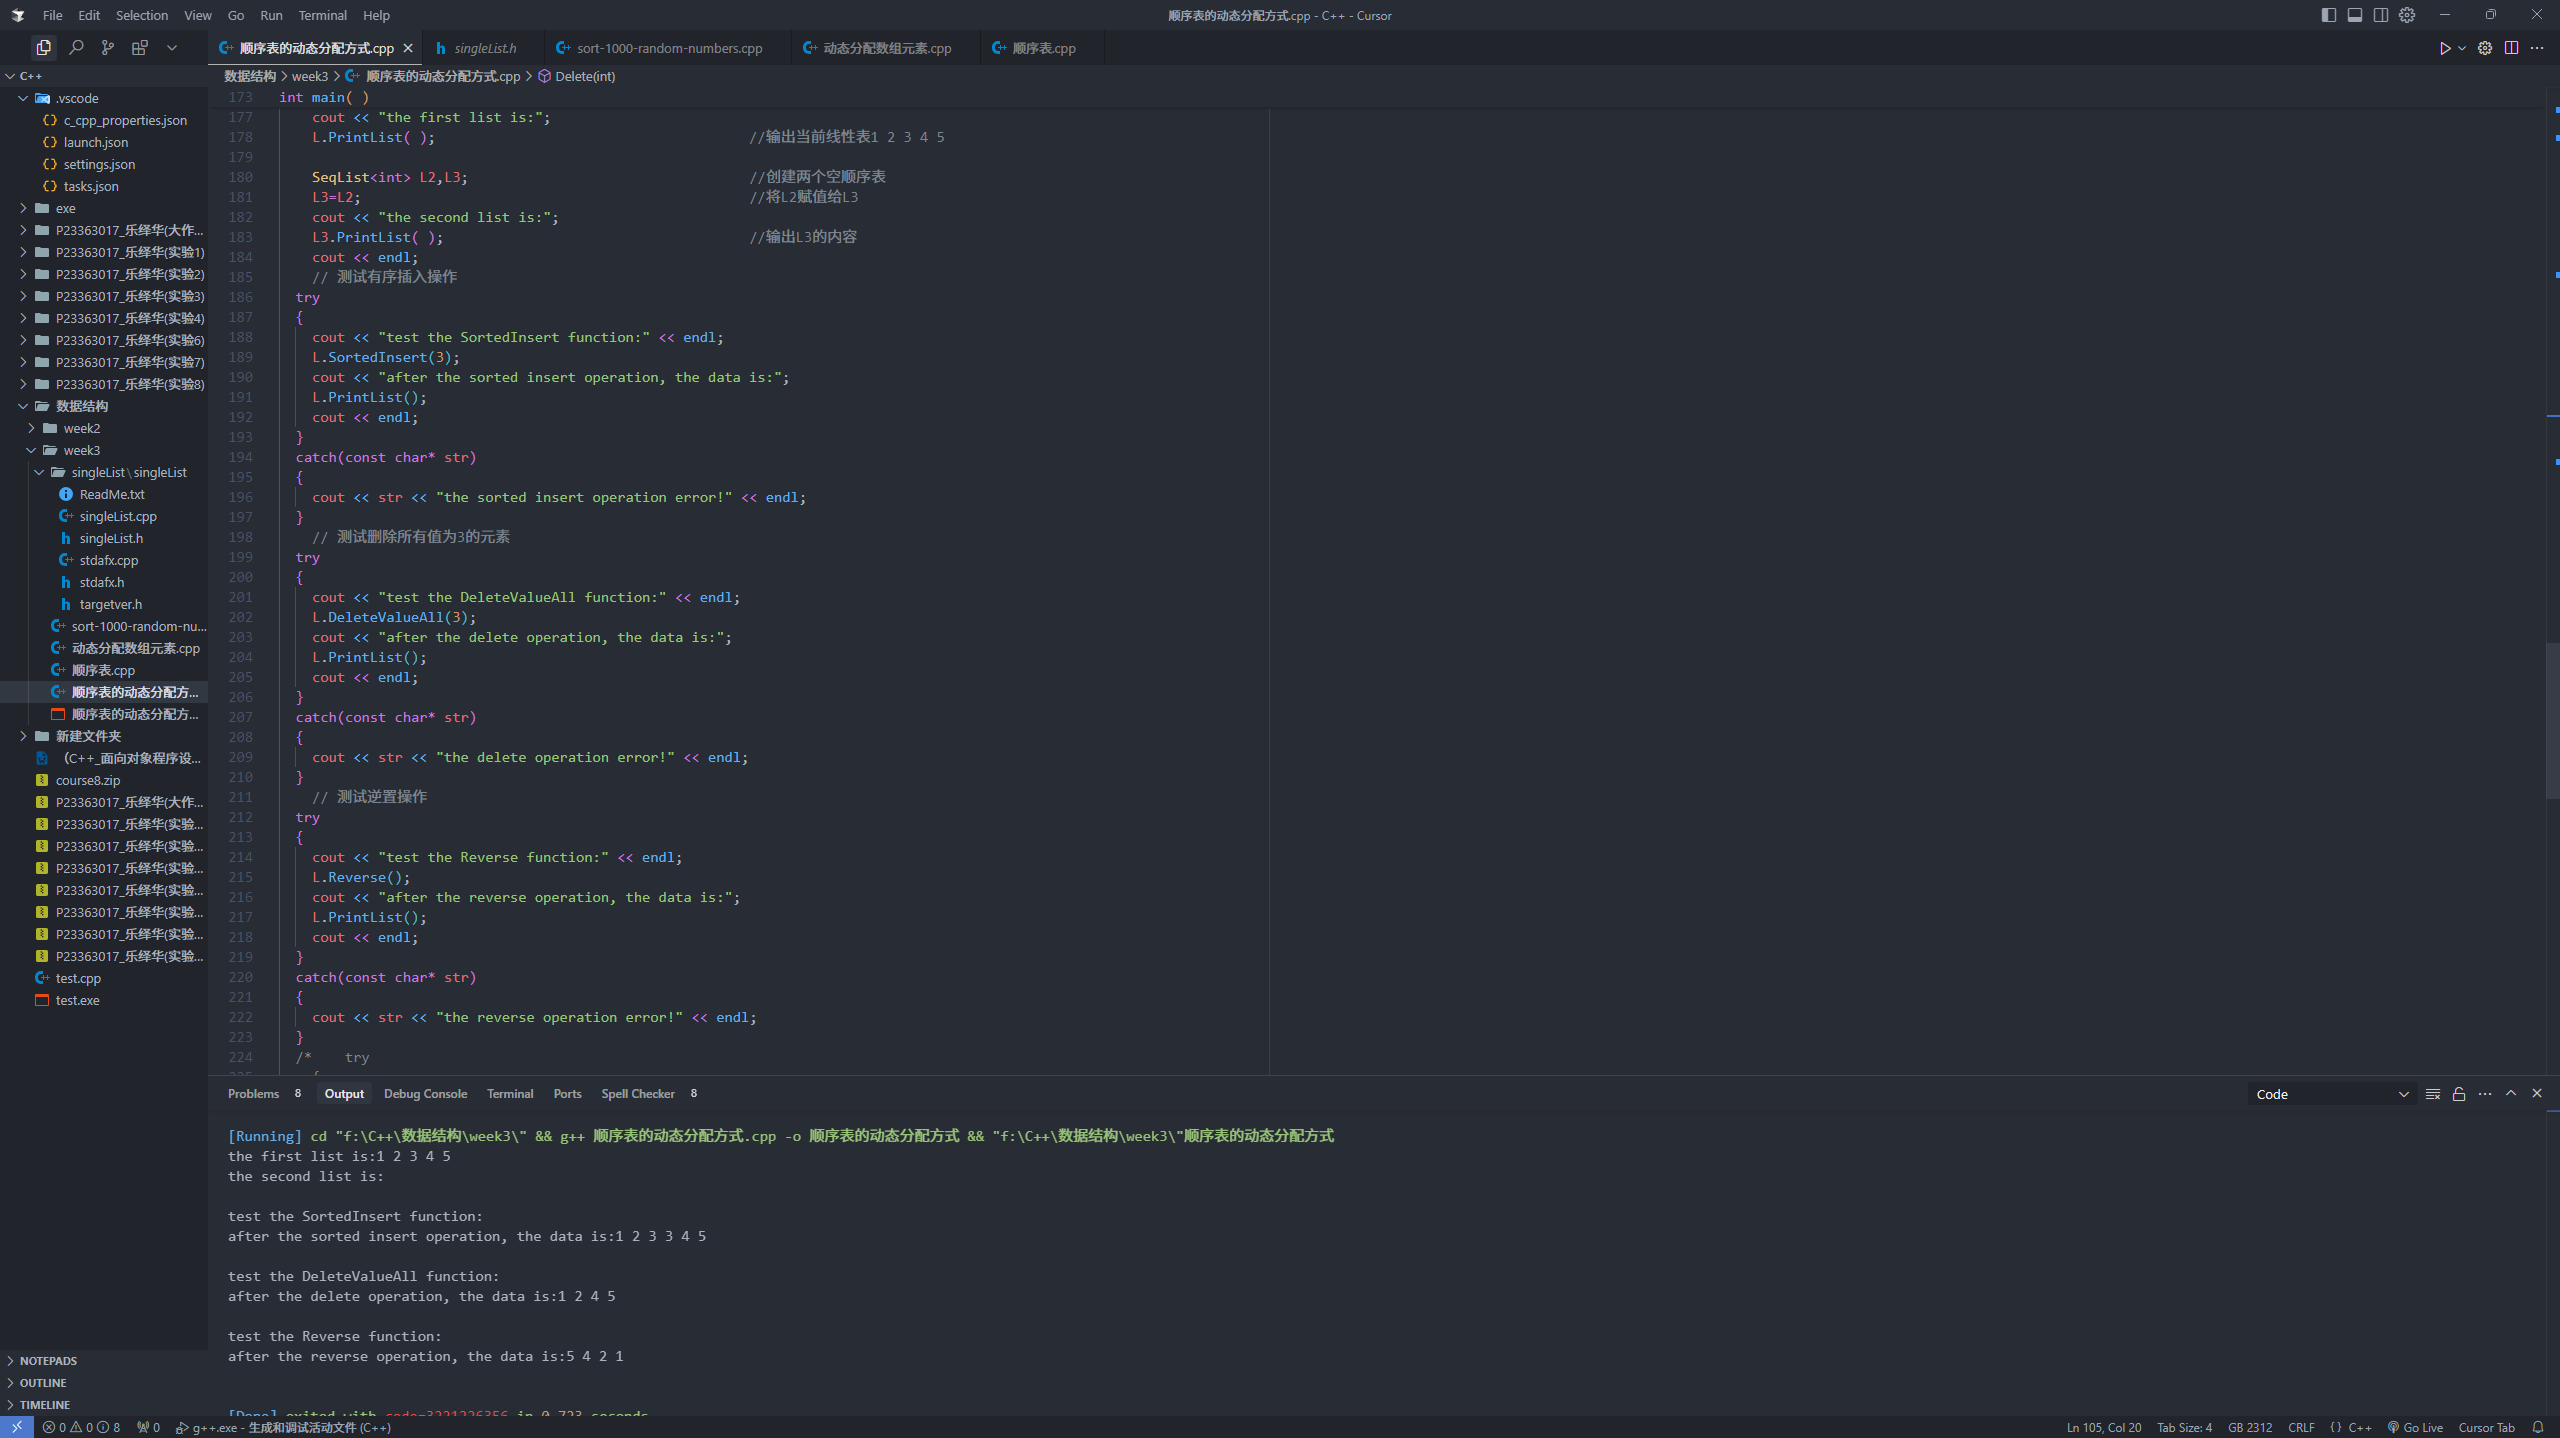
\includegraphics[width=\textwidth]{2-实验报告3-20250317.png}
% \caption{}
\label{}
\end{figure}

\section{10000 个数据通过顺序表来排序}

\begin{lstlisting}[language=C++]
//2.(选做)生成10000个随机数,保存都数据文件中,使用顺序表存贮,调用不同的排序方法,排序后结果保存到数据文件ResultSorted.txt中。

  

#include <iostream>

#include <ctime>    // 添加 ctime 头文件

#include <fstream>  // 添加 fstream 头文件

using namespace std;

  

const int MaxSize = 10000;            //修改为10000以支持更多数据

template <class DataType>          //定义模板类SeqList

class SeqList

{

public:

    SeqList( );                     //无参构造函数,建立空的顺序表

    SeqList(DataType a[ ], int n);      //有参构造函数,建立长度为n的顺序表

    ~SeqList( );                    //析构函数

    int Length( );                   //求线性表的长度

    int Empety();                    //判断线性表是否为空

    DataType Get(int i);              //按位查找,查找第i个元素的值

    int Locate(DataType x );          //按值查找,查找值为x的元素序号

    void Insert(int i, DataType x);      //插入操作,在第i个位置插入值为x的元素

    DataType Delete(int i);            //删除操作,删除第i个元素

    void PrintList( );                 //遍历操作,按序号依次输出各元素

    void Reverse( );               //**将顺序表逆置,实验书p37

    void Insert(DataType x);         //**在有序顺序表中插入操作x的元素,并保持表L仍递增有序

    void Swap(int i, int j);          //交换两个位置的元素

    //void Delete(DataType x);        //**这样不行,不能重载,在顺序表中删除所有元素值为x的元素,要求空间复杂度为O(1)

    DataType *GetSeqList() ;         //获取顺序表数组指针

    template <class T> friend void Delete1(SeqList<T> &L, T x);        //**在顺序表中删除所有元素值为x的元素,要求空间复杂度为O(1)

    template <class T> friend void Delete2(T a[MaxSize], T x);        //**在顺序表中删除所有元素值为x的元素,要求空间复杂度为O(1)

  private:

    DataType data[MaxSize];          //存放数据元素的数组

    int length;                       //线性表的长度

};

  

template<class DataType>

SeqList<DataType> :: ~SeqList()

{

    // 析构函数,不需要做任何事情,因为data是静态数组    

}

  

template<class DataType>

DataType *SeqList<DataType> :: GetSeqList()

{

  return data;  // 返回数组指针,用于外部访问

}

template <class DataType>

SeqList<DataType> :: SeqList()

{

    length = 0;  // 初始化空顺序表,长度为0

}

  

template <class DataType>

int SeqList<DataType> :: Empety()

{

    if(length == 0)  // 判断顺序表是否为空

        return 1;    // 为空返回1

    else

        return 0;    // 不为空返回0

}

  

template <class DataType>

int SeqList<DataType> :: Length()

{

  // 返回顺序表的长度

  return length;

}

  

template <class DataType>  

SeqList<DataType> :: SeqList(DataType a[ ], int n)

{

    if (n > MaxSize)  // 检查参数合法性

        throw "参数非法";

    for (int i = 0; i < n; i++)  // 复制数组元素到顺序表

        data[i] = a[i];

    length = n;  // 设置顺序表长度

}

  

template <class DataType>  

void SeqList<DataType> :: PrintList( )

{

    for (int i = 0; i < length; i++)  // 遍历顺序表

        cout << data[i]<<" ";         // 依次输出线性表的元素值

}

  

template <class DataType>  

int SeqList<DataType> :: Locate(DataType x)

{

    for (int i = 0; i < length; i++)  // 遍历顺序表

        if (data[i] == x) return i+1;  // 找到元素x,返回其序号i+1

    return 0;                         // 退出循环,说明查找失败

}

  

template <class DataType>  

DataType SeqList<DataType> :: Get(int i)

{

    if (i < 0 || i >= length)  // 修改索引检查条件

        throw "查找位置非法";

    else

        return data[i];  // 直接返回数组元素

}

  

template <class DataType>  

DataType SeqList<DataType> :: Delete(int i)

{

    if (length == 0)  // 检查是否为空表

        throw "下溢";

    if (i < 1 || i > length)  // 检查位置是否合法

        throw "位置";

    int x = data[i - 1];      // 取出位置i的元素

    for (int j = i; j < length; j++)  // 将后面的元素前移

        data[j - 1] = data[j];       // 此处j已经是元素所在的数组下标

    length--;  // 长度减1

    return x;  // 返回被删除的元素

}

  

template <class DataType>  

void SeqList<DataType> :: Insert(int i, DataType x)

{

    if (length >= MaxSize)  // 检查是否已满

        throw "上溢";

    if (i < 1 || i > length + 1)  // 检查位置是否合法

        throw "位置";

    for (int j = length; j >= i; j--)  // 将元素后移

        data[j] = data[j - 1];        // 第j个元素存在数组下标为j-1处

    data[i - 1] = x;  // 在位置i插入新元素

    length++;  // 长度加1

}

  
  

template <class DataType>   //**顺序表逆序  

void SeqList<DataType> :: Reverse()

{  

  // 实现顺序表的逆置操作

  DataType temp;

  for(int i = 0; i < length/2; i++) {

    temp = data[i];

    data[i] = data[length-1-i];

    data[length-1-i] = temp;

  }

}

  

template <class DataType>   //**在有序顺序表中插入x  

void SeqList<DataType> :: Insert(DataType x)

{  

  // 在有序顺序表中插入元素x,保持有序性

  int i;

  if(length >= MaxSize)  // 检查是否已满

    throw "上溢";

  // 找到插入位置

  for(i = 0; i < length; i++) {

    if(data[i] > x)

      break;

  }

  // 将元素后移

  for(int j = length; j > i; j--)

    data[j] = data[j-1];

  data[i] = x;  // 插入新元素

  length++;  // 长度加1

}

  

/*template <class DataType>   //**这样不行,不能重载删除所有元素值为x的元素  

void SeqList<DataType>::Delete(DataType x)

{  

  

}*/

  

template <class DataType>   //**用普通函数实现,删除所有元素值为x的元素

void Delete1(SeqList<DataType> &L, DataType x)

{

  // 删除顺序表L中所有值为x的元素

  int k = 0;  // k记录不等于x的元素个数

  for(int i = 0; i < L.length; i++) {

    if(L.data[i] != x) {  // 如果当前元素不等于x

      L.data[k] = L.data[i];  // 保留该元素

      k++;  // 不等于x的元素计数加1

    }

  }

  L.length = k;  // 更新顺序表长度

}

  

template <class T>   //**用普通函数实现,删除所有元素值为x的元素

void Delete2(T a[MaxSize], T x)  

{

  // 这个函数需要知道数组的实际长度才能正确工作

  // 由于参数中没有提供长度信息,此函数实现可能不完整

  // 实际使用时需要传入长度参数或者在数组中标记结束

}

  

template <class DataType>

void SeqList<DataType>::Swap(int i, int j) {

    DataType temp = data[i];

    data[i] = data[j];

    data[j] = temp;

}

  

// 函数声明

void create(int *r, int n);

void print(int *r, int n);

  

// 冒泡排序

void BubbleSort(SeqList<int> &L)

{

  // 冒泡排序实现

  for (int i = 0; i < L.Length() - 1; i++) {

    for (int j = 0; j < L.Length() - i - 1; j++) {

      if (L.Get(j) > L.Get(j + 1)) {

        L.Swap(j, j + 1);

      }

    }

  }

}

  

// 选择排序

void SelectionSort(SeqList<int> &L)

{

  // 选择排序实现

  for (int i = 0; i < L.Length() - 1; i++) {

    int minIndex = i;

    for (int j = i + 1; j < L.Length(); j++) {

      if (L.Get(j) < L.Get(minIndex)) {

        minIndex = j;

      }

    }

    if (minIndex != i) {

      L.Swap(i, minIndex);

    }

  }

}

  
  
  
  

// 2.(选做)生成10000个随机数,保存都数据文件中,使用顺序表存贮,调用不同的排序方法,排序后结果保存到数据文件ResultSorted.txt中。

  

int main( )

{

    int n = 10000;

    int *a = NULL;

    a = new int[n];

    create(a, n);

    // print(a, n);

    // 存储到数据文件中

    ofstream outFile("data.txt");

    if (!outFile) {

        cout << "无法打开文件" << endl;

        return 1;

    }

    for (int i = 0; i < n; i++) {

        outFile << a[i] << " ";

    }

    outFile.close();

  

    // 用顺序表存储

    SeqList<int> L(a, n);

    // 冒泡排序

    BubbleSort(L);

    ofstream outFile2("ResultSorted.txt");

    if (!outFile2) {

        cout << "无法打开文件" << endl;

        return 1;

    }

    for (int i = 0; i < n; i++) {

        outFile2 << L.Get(i) << " ";

    }

    outFile2.close();

    // 选择排序

    SelectionSort(L);

    int *b = NULL;

    b = new int[n];

    for (int i = 0; i < n; i++) {

        b[i] = L.Get(i);

    }

    ofstream outFile3("ResultSorted2.txt");

    if (!outFile3) {

        cout << "无法打开文件" << endl;

        return 1;

    }

    for (int i = 0; i < n; i++) {

        outFile3 << b[i] << " ";

    }

    outFile3.close();

  
  
  
  
  
  
  

    return 0;  //程序正常结束

}

  

// 创建随机数组的函数实现

void create(int *r, int n)

{

    int i = 0;

    srand(time(NULL));              // 初始化随机数生成器

    for (i = 0; i < n; i++)         // 遍历数组

        *(r+i) =1+ rand() ;    // 使用指针算术生成1到100的随机数

}

  

// 打印数组元素的函数实现

void print(int *r, int n)

{

    int i = 0;

    for (i = 0; i < n; i++)         // 遍历数组

    cout<<*(r+i)<<"  ";             // 使用指针算术输出数组元素

}
\end{lstlisting}
\begin{figure}[H]
\centering
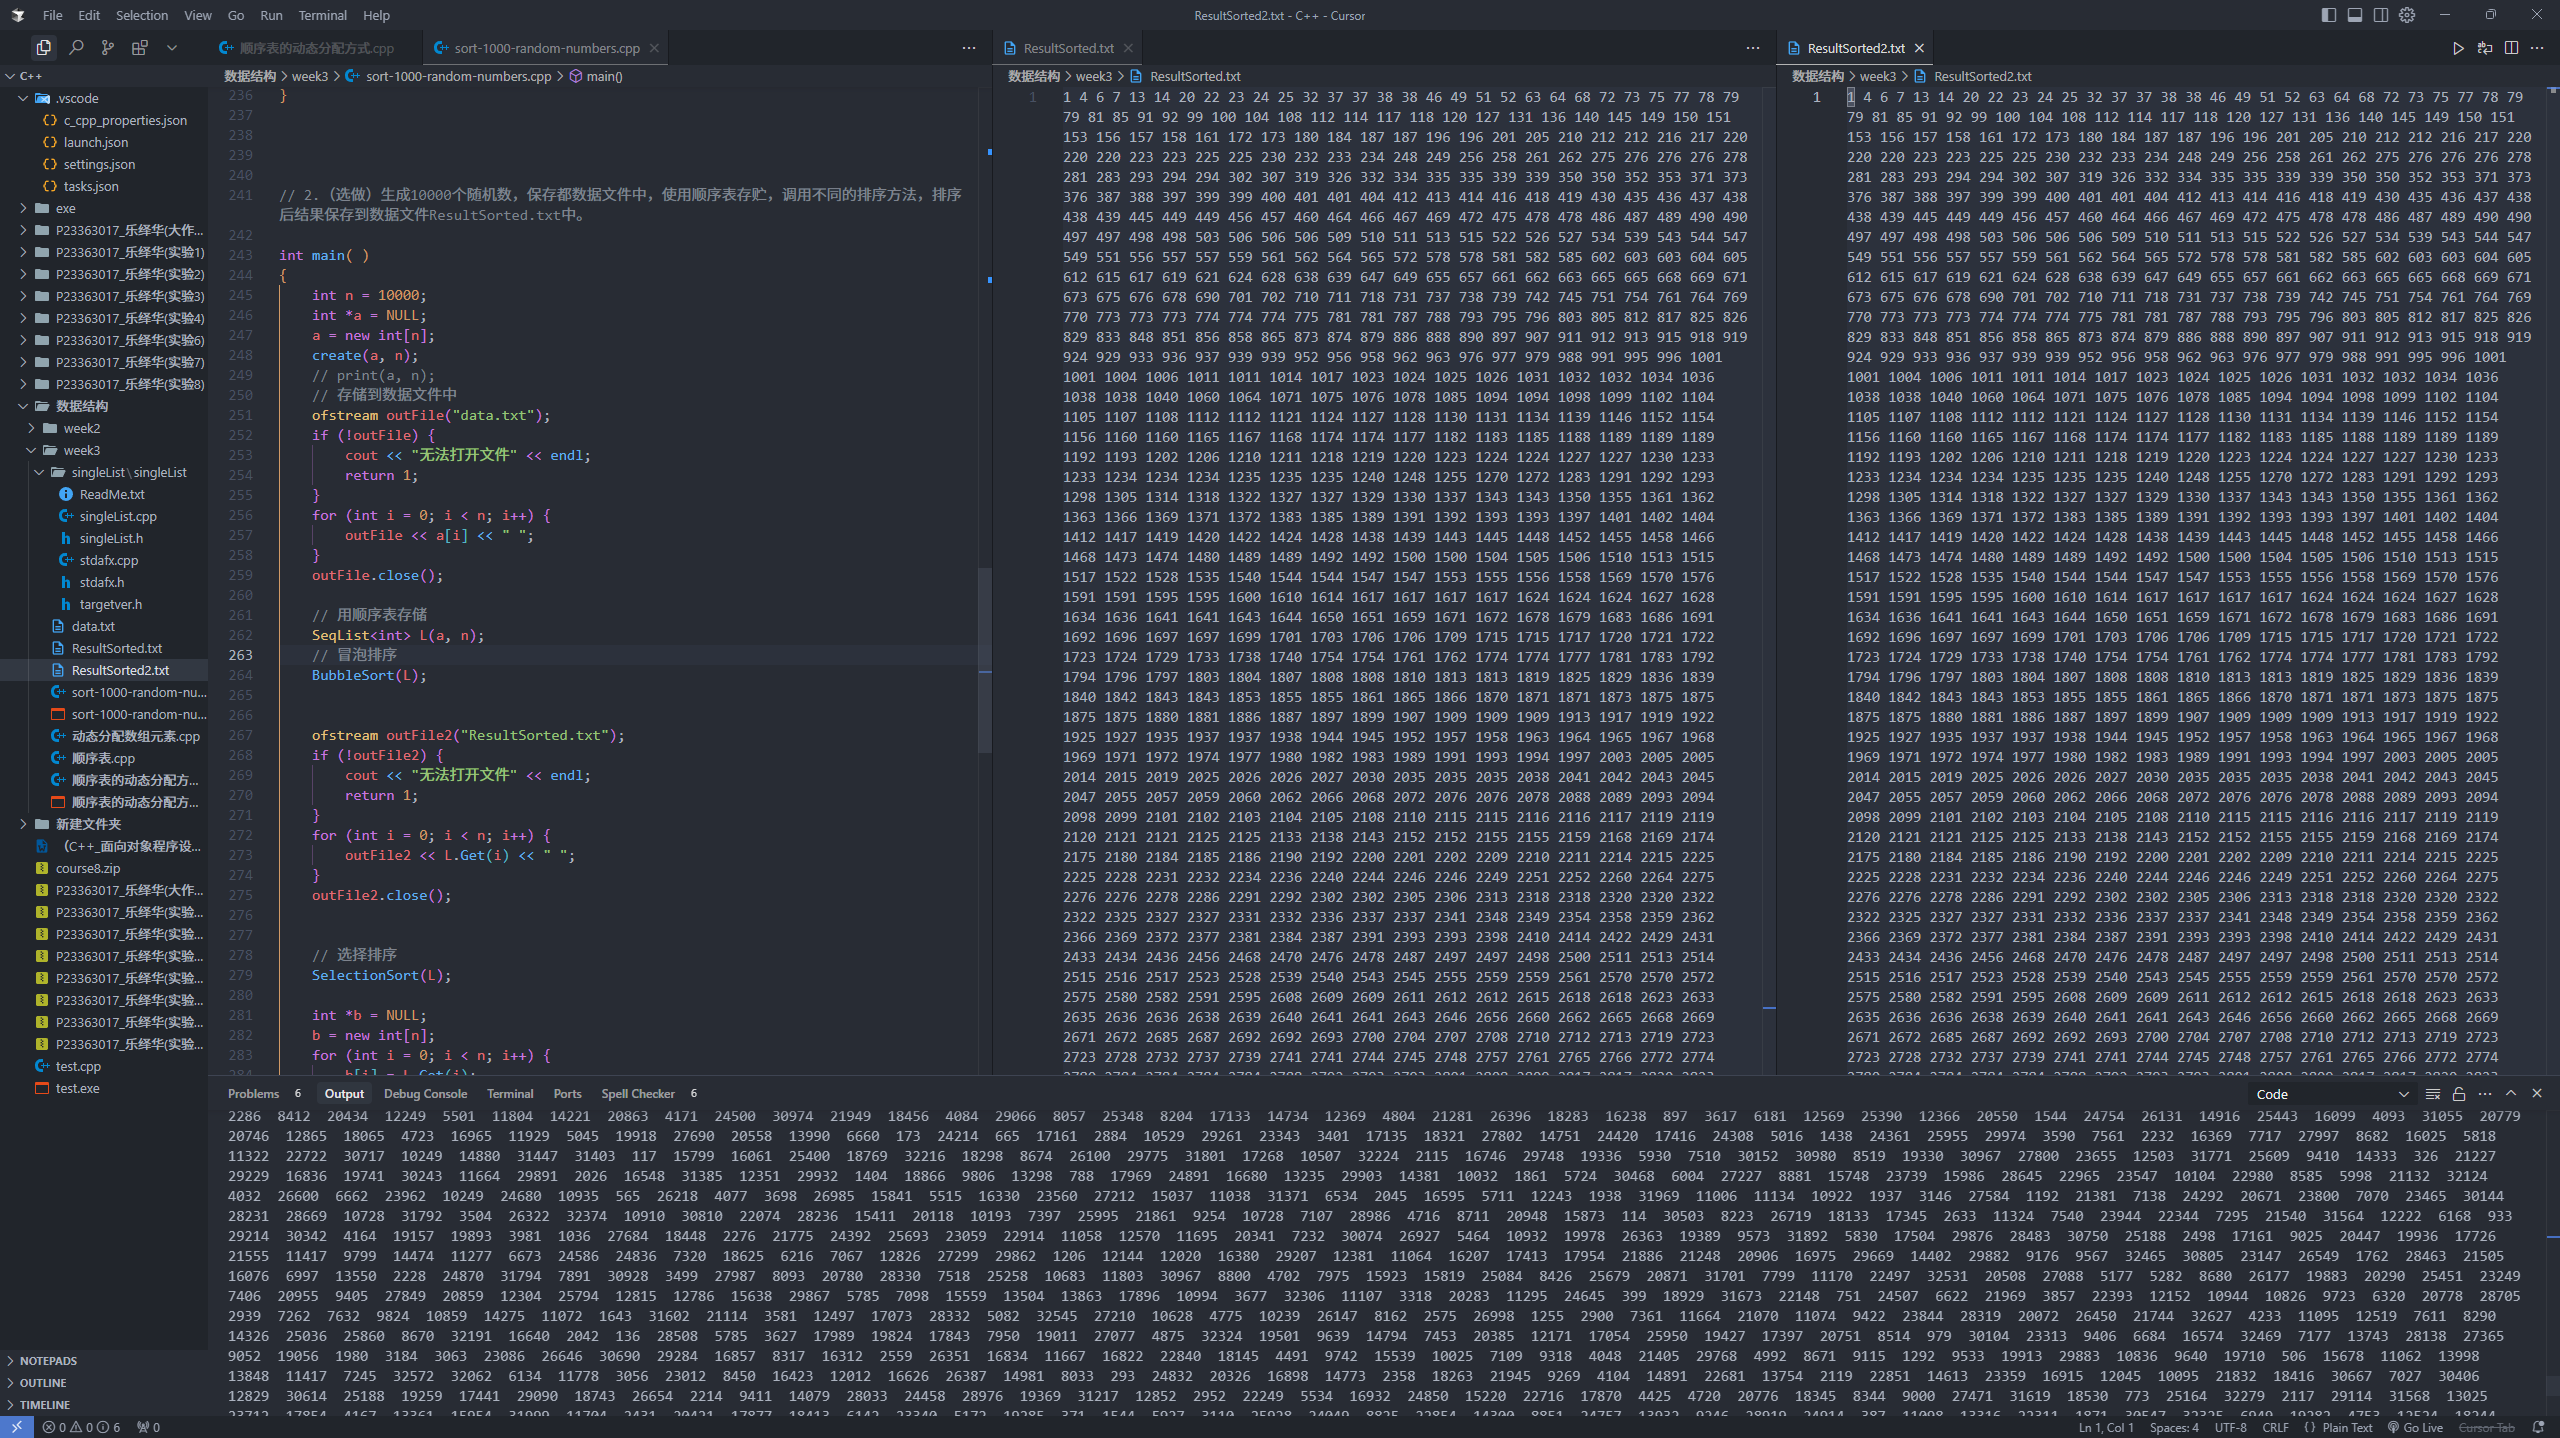
\includegraphics[width=\textwidth]{3-实验报告3-20250317.png}
% \caption{}
\label{}
\end{figure}

先造出了 10000 个随机数,并存储到 \lstinline{data.txt} 文件中,然后将这 10000 个数据通过冒泡排序生成从小到大的顺序的数据,存储到 \lstinline{ResultSorted.txt} 中。再生成 10000 个随机数,通过选择排序,将排好序的数据存储到 \lstinline{ResultSorted2.txt} 中。
